\documentclass[twoside]{book}

% Packages required by doxygen
\usepackage{fixltx2e}
\usepackage{calc}
\usepackage{doxygen}
\usepackage[export]{adjustbox} % also loads graphicx
\usepackage{graphicx}
\usepackage[utf8]{inputenc}
\usepackage{makeidx}
\usepackage{multicol}
\usepackage{multirow}
\PassOptionsToPackage{warn}{textcomp}
\usepackage{textcomp}
\usepackage[nointegrals]{wasysym}
\usepackage[table]{xcolor}

% Font selection
\usepackage[T1]{fontenc}
\usepackage[scaled=.90]{helvet}
\usepackage{courier}
\usepackage{amssymb}
\usepackage{sectsty}
\renewcommand{\familydefault}{\sfdefault}
\allsectionsfont{%
  \fontseries{bc}\selectfont%
  \color{darkgray}%
}
\renewcommand{\DoxyLabelFont}{%
  \fontseries{bc}\selectfont%
  \color{darkgray}%
}
\newcommand{\+}{\discretionary{\mbox{\scriptsize$\hookleftarrow$}}{}{}}

% Page & text layout
\usepackage{geometry}
\geometry{%
  a4paper,%
  top=2.5cm,%
  bottom=2.5cm,%
  left=2.5cm,%
  right=2.5cm%
}
\tolerance=750
\hfuzz=15pt
\hbadness=750
\setlength{\emergencystretch}{15pt}
\setlength{\parindent}{0cm}
\setlength{\parskip}{3ex plus 2ex minus 2ex}
\makeatletter
\renewcommand{\paragraph}{%
  \@startsection{paragraph}{4}{0ex}{-1.0ex}{1.0ex}{%
    \normalfont\normalsize\bfseries\SS@parafont%
  }%
}
\renewcommand{\subparagraph}{%
  \@startsection{subparagraph}{5}{0ex}{-1.0ex}{1.0ex}{%
    \normalfont\normalsize\bfseries\SS@subparafont%
  }%
}
\makeatother

% Headers & footers
\usepackage{fancyhdr}
\pagestyle{fancyplain}
\fancyhead[LE]{\fancyplain{}{\bfseries\thepage}}
\fancyhead[CE]{\fancyplain{}{}}
\fancyhead[RE]{\fancyplain{}{\bfseries\leftmark}}
\fancyhead[LO]{\fancyplain{}{\bfseries\rightmark}}
\fancyhead[CO]{\fancyplain{}{}}
\fancyhead[RO]{\fancyplain{}{\bfseries\thepage}}
\fancyfoot[LE]{\fancyplain{}{}}
\fancyfoot[CE]{\fancyplain{}{}}
\fancyfoot[RE]{\fancyplain{}{\bfseries\scriptsize Generated by Doxygen }}
\fancyfoot[LO]{\fancyplain{}{\bfseries\scriptsize Generated by Doxygen }}
\fancyfoot[CO]{\fancyplain{}{}}
\fancyfoot[RO]{\fancyplain{}{}}
\renewcommand{\footrulewidth}{0.4pt}
\renewcommand{\chaptermark}[1]{%
  \markboth{#1}{}%
}
\renewcommand{\sectionmark}[1]{%
  \markright{\thesection\ #1}%
}

% Indices & bibliography
\usepackage{natbib}
\usepackage[titles]{tocloft}
\setcounter{tocdepth}{3}
\setcounter{secnumdepth}{5}
\makeindex

% Hyperlinks (required, but should be loaded last)
\usepackage{ifpdf}
\ifpdf
  \usepackage[pdftex,pagebackref=true]{hyperref}
\else
  \usepackage[ps2pdf,pagebackref=true]{hyperref}
\fi
\hypersetup{%
  colorlinks=true,%
  linkcolor=blue,%
  citecolor=blue,%
  unicode%
}

% Custom commands
\newcommand{\clearemptydoublepage}{%
  \newpage{\pagestyle{empty}\cleardoublepage}%
}

\usepackage{caption}
\captionsetup{labelsep=space,justification=centering,font={bf},singlelinecheck=off,skip=4pt,position=top}

%===== C O N T E N T S =====

\begin{document}

% Titlepage & ToC
\hypersetup{pageanchor=false,
             bookmarksnumbered=true,
             pdfencoding=unicode
            }
\pagenumbering{roman}
\begin{titlepage}
\vspace*{7cm}
\begin{center}%
{\Large My Project }\\
\vspace*{1cm}
{\large Generated by Doxygen 1.8.11}\\
\end{center}
\end{titlepage}
\clearemptydoublepage
\tableofcontents
\clearemptydoublepage
\pagenumbering{arabic}
\hypersetup{pageanchor=true}

%--- Begin generated contents ---
\chapter{Projet\+\_\+impl-\/mentation\+\_\+\+Wakanda}
\label{md_README}
\hypertarget{md_README}{}
Ce projet consiste à asservir un robot parallèle.

Nous utilisons une Beaglebone Black, un pont en H ainsi que 2 encodeurs connectés à 2 moteurs. Le contrôle de ces deux moteurs se fait grâce à deux P\+ID (un pour chaque moteur)

Pour tester l\textquotesingle{}asservissement, lancer le fichier \char`\"{}wakanda.\+py\char`\"{} 
\chapter{Hierarchical Index}
\section{Class Hierarchy}
This inheritance list is sorted roughly, but not completely, alphabetically\+:\begin{DoxyCompactList}
\item object\begin{DoxyCompactList}
\item \contentsline{section}{eqep.\+e\+Q\+EP}{\pageref{classeqep_1_1eQEP}}{}
\item \contentsline{section}{pwm.\+P\+WM}{\pageref{classpwm_1_1PWM}}{}
\item \contentsline{section}{wakanda.\+Wakanda}{\pageref{classwakanda_1_1Wakanda}}{}
\end{DoxyCompactList}
\item Thread\begin{DoxyCompactList}
\item \contentsline{section}{controller.\+Controller}{\pageref{classcontroller_1_1Controller}}{}
\end{DoxyCompactList}
\end{DoxyCompactList}

\chapter{Class Index}
\section{Class List}
Here are the classes, structs, unions and interfaces with brief descriptions\+:\begin{DoxyCompactList}
\item\contentsline{section}{\hyperlink{classcontroller_1_1Controller}{controller.\+Controller} \\*Classe permettant de controler les moteurs grace a un P\+ID (un P\+ID pour chaque moteur) }{\pageref{classcontroller_1_1Controller}}{}
\item\contentsline{section}{\hyperlink{classeqep_1_1eQEP}{eqep.\+e\+Q\+EP} \\*Classe permettant de gerer la position du moteur }{\pageref{classeqep_1_1eQEP}}{}
\item\contentsline{section}{\hyperlink{classpwm_1_1PWM}{pwm.\+P\+WM} \\*Classe permettant de gerer le module \hyperlink{classpwm_1_1PWM}{P\+WM} }{\pageref{classpwm_1_1PWM}}{}
\item\contentsline{section}{\hyperlink{classwakanda_1_1Wakanda}{wakanda.\+Wakanda} \\*Classe principale responsable du suivi de trajectoire }{\pageref{classwakanda_1_1Wakanda}}{}
\end{DoxyCompactList}

\chapter{Class Documentation}
\hypertarget{classcontroller_1_1Controller}{}\section{controller.\+Controller Class Reference}
\label{classcontroller_1_1Controller}\index{controller.\+Controller@{controller.\+Controller}}


Classe permettant de controler les moteurs grace a un P\+ID (un P\+ID pour chaque moteur)  




Inheritance diagram for controller.\+Controller\+:\nopagebreak
\begin{figure}[H]
\begin{center}
\leavevmode
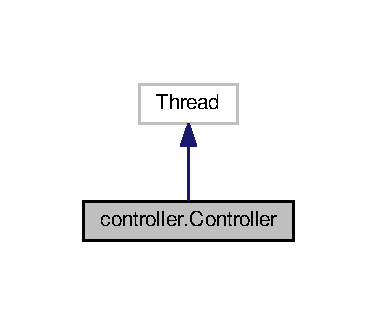
\includegraphics[width=181pt]{classcontroller_1_1Controller__inherit__graph}
\end{center}
\end{figure}


Collaboration diagram for controller.\+Controller\+:\nopagebreak
\begin{figure}[H]
\begin{center}
\leavevmode
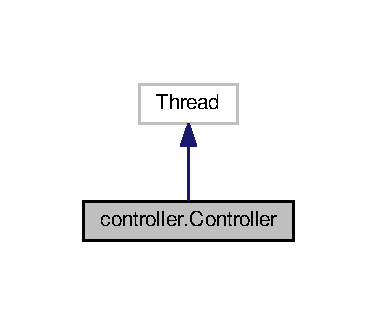
\includegraphics[width=181pt]{classcontroller_1_1Controller__coll__graph}
\end{center}
\end{figure}
\subsection*{Public Member Functions}
\begin{DoxyCompactItemize}
\item 
def \hyperlink{classcontroller_1_1Controller_a60886a7a74662e1d71da2e88555bb08b}{\+\_\+\+\_\+init\+\_\+\+\_\+} (self, pin\+P\+W\+M1, pin\+Dir1, pin\+P\+W\+M2, pin\+Dir2)
\begin{DoxyCompactList}\small\item\em Constructeur, on va y initialiser les pins pour le P\+WM et pour la direction pour chaque moteur. \end{DoxyCompactList}\item 
def \hyperlink{classcontroller_1_1Controller_a93cb1a5ccca3ca00f803da3558dee95d}{send\+Cmd} (self, motor, val)
\begin{DoxyCompactList}\small\item\em Envoie la commande entrée en argument a un moteur. \end{DoxyCompactList}\item 
def \hyperlink{classcontroller_1_1Controller_aea95f1e9b68ed4eb5447e3e4aed805fa}{execute} (self)\hypertarget{classcontroller_1_1Controller_aea95f1e9b68ed4eb5447e3e4aed805fa}{}\label{classcontroller_1_1Controller_aea95f1e9b68ed4eb5447e3e4aed805fa}

\begin{DoxyCompactList}\small\item\em Calcule la valeur de la commande a envoyer grace a un P\+ID. \end{DoxyCompactList}\item 
def \hyperlink{classcontroller_1_1Controller_a8ba4b15d12681e8f94bfa136d984f8a4}{stop} (self)\hypertarget{classcontroller_1_1Controller_a8ba4b15d12681e8f94bfa136d984f8a4}{}\label{classcontroller_1_1Controller_a8ba4b15d12681e8f94bfa136d984f8a4}

\begin{DoxyCompactList}\small\item\em Arrete les deux moteurs. \end{DoxyCompactList}\item 
def \hyperlink{classcontroller_1_1Controller_a49d765b2942b1631d4c2680f2864fd55}{set\+Des} (self, val1, val2)
\begin{DoxyCompactList}\small\item\em Definit une nouvelle position angulaire a atteindre pour les deux moteurs. \end{DoxyCompactList}\item 
def \hyperlink{classcontroller_1_1Controller_a6a29180c5d05fe547cd94cc9074af539}{regulate\+Cmd} (self, motor, cmd)
\begin{DoxyCompactList}\small\item\em Effectue la regulation des commandes a envoyer a un moteur en les mettant sous forme de pourcentage. \end{DoxyCompactList}\end{DoxyCompactItemize}
\subsection*{Public Attributes}
\begin{DoxyCompactItemize}
\item 
{\bfseries encoder1}\hypertarget{classcontroller_1_1Controller_a5b8777fdb2c8ad7684384109c392166c}{}\label{classcontroller_1_1Controller_a5b8777fdb2c8ad7684384109c392166c}

\item 
{\bfseries encoder2}\hypertarget{classcontroller_1_1Controller_a1f360500a110c27d8e0163fe2122a51c}{}\label{classcontroller_1_1Controller_a1f360500a110c27d8e0163fe2122a51c}

\item 
{\bfseries pin\+P\+W\+M1}\hypertarget{classcontroller_1_1Controller_a24253a87e72aac6cd3b3a786ad2a3224}{}\label{classcontroller_1_1Controller_a24253a87e72aac6cd3b3a786ad2a3224}

\item 
{\bfseries pin\+Dir1}\hypertarget{classcontroller_1_1Controller_af30aeb66aaf7f9bd9e795fc5692e7fbe}{}\label{classcontroller_1_1Controller_af30aeb66aaf7f9bd9e795fc5692e7fbe}

\item 
{\bfseries pin\+P\+W\+M2}\hypertarget{classcontroller_1_1Controller_a12984a4e33d79c394371931404318e6f}{}\label{classcontroller_1_1Controller_a12984a4e33d79c394371931404318e6f}

\item 
{\bfseries pin\+Dir2}\hypertarget{classcontroller_1_1Controller_ad640b792986fc8ad08b3e44e00beff3c}{}\label{classcontroller_1_1Controller_ad640b792986fc8ad08b3e44e00beff3c}

\item 
{\bfseries P\+WM}\hypertarget{classcontroller_1_1Controller_a0fdc67cb88248e25bea07b88ee790caa}{}\label{classcontroller_1_1Controller_a0fdc67cb88248e25bea07b88ee790caa}

\item 
{\bfseries G\+P\+IO}\hypertarget{classcontroller_1_1Controller_a1833635d6e43c51d1575dd148aba2416}{}\label{classcontroller_1_1Controller_a1833635d6e43c51d1575dd148aba2416}

\item 
{\bfseries Kp}\hypertarget{classcontroller_1_1Controller_a34cf377d78ee193d7160d74adbe9aabf}{}\label{classcontroller_1_1Controller_a34cf377d78ee193d7160d74adbe9aabf}

\item 
{\bfseries Kd}\hypertarget{classcontroller_1_1Controller_aa67f4d0fe3cb5e3659bf036eaa44f246}{}\label{classcontroller_1_1Controller_aa67f4d0fe3cb5e3659bf036eaa44f246}

\item 
{\bfseries Ki}\hypertarget{classcontroller_1_1Controller_ae2cdbac964e61042bab697b094df1e02}{}\label{classcontroller_1_1Controller_ae2cdbac964e61042bab697b094df1e02}

\item 
{\bfseries last\+Error1}\hypertarget{classcontroller_1_1Controller_a5b83374cef792121cf491db65eb4f722}{}\label{classcontroller_1_1Controller_a5b83374cef792121cf491db65eb4f722}

\item 
{\bfseries total\+Error1}\hypertarget{classcontroller_1_1Controller_a6f90d9dd72798c3d4e4fe7da9854f577}{}\label{classcontroller_1_1Controller_a6f90d9dd72798c3d4e4fe7da9854f577}

\item 
{\bfseries last\+Error2}\hypertarget{classcontroller_1_1Controller_af360e38aa896ac13078d88207b5d2ac1}{}\label{classcontroller_1_1Controller_af360e38aa896ac13078d88207b5d2ac1}

\item 
{\bfseries total\+Error2}\hypertarget{classcontroller_1_1Controller_a38ea8aa69fc02a699ee30b932f02afa4}{}\label{classcontroller_1_1Controller_a38ea8aa69fc02a699ee30b932f02afa4}

\item 
{\bfseries des1}\hypertarget{classcontroller_1_1Controller_a98214ada766afa8f1312bdcce1b21983}{}\label{classcontroller_1_1Controller_a98214ada766afa8f1312bdcce1b21983}

\item 
{\bfseries des2}\hypertarget{classcontroller_1_1Controller_a9600b6cbf89f06afeb5f19bc6b51bbc7}{}\label{classcontroller_1_1Controller_a9600b6cbf89f06afeb5f19bc6b51bbc7}

\end{DoxyCompactItemize}


\subsection{Detailed Description}
Classe permettant de controler les moteurs grace a un P\+ID (un P\+ID pour chaque moteur) 

\subsection{Constructor \& Destructor Documentation}
\index{controller\+::\+Controller@{controller\+::\+Controller}!\+\_\+\+\_\+init\+\_\+\+\_\+@{\+\_\+\+\_\+init\+\_\+\+\_\+}}
\index{\+\_\+\+\_\+init\+\_\+\+\_\+@{\+\_\+\+\_\+init\+\_\+\+\_\+}!controller\+::\+Controller@{controller\+::\+Controller}}
\subsubsection[{\texorpdfstring{\+\_\+\+\_\+init\+\_\+\+\_\+(self, pin\+P\+W\+M1, pin\+Dir1, pin\+P\+W\+M2, pin\+Dir2)}{__init__(self, pinPWM1, pinDir1, pinPWM2, pinDir2)}}]{\setlength{\rightskip}{0pt plus 5cm}def controller.\+Controller.\+\_\+\+\_\+init\+\_\+\+\_\+ (
\begin{DoxyParamCaption}
\item[{}]{self, }
\item[{}]{pin\+P\+W\+M1, }
\item[{}]{pin\+Dir1, }
\item[{}]{pin\+P\+W\+M2, }
\item[{}]{pin\+Dir2}
\end{DoxyParamCaption}
)}\hypertarget{classcontroller_1_1Controller_a60886a7a74662e1d71da2e88555bb08b}{}\label{classcontroller_1_1Controller_a60886a7a74662e1d71da2e88555bb08b}


Constructeur, on va y initialiser les pins pour le P\+WM et pour la direction pour chaque moteur. 


\begin{DoxyParams}{Parameters}
{\em pin\+P\+W\+M1} & Le pin de P\+WM du moteur 1 \\
\hline
{\em pin\+Dir1} & Le pin de direction du moteur 1 \\
\hline
{\em pin\+P\+W\+M2} & Le pin de P\+WM du moteur 2 \\
\hline
{\em pin\+Dir2} & Le pin de direction du moteur 2 \\
\hline
\end{DoxyParams}


\subsection{Member Function Documentation}
\index{controller\+::\+Controller@{controller\+::\+Controller}!regulate\+Cmd@{regulate\+Cmd}}
\index{regulate\+Cmd@{regulate\+Cmd}!controller\+::\+Controller@{controller\+::\+Controller}}
\subsubsection[{\texorpdfstring{regulate\+Cmd(self, motor, cmd)}{regulateCmd(self, motor, cmd)}}]{\setlength{\rightskip}{0pt plus 5cm}def controller.\+Controller.\+regulate\+Cmd (
\begin{DoxyParamCaption}
\item[{}]{self, }
\item[{}]{motor, }
\item[{}]{cmd}
\end{DoxyParamCaption}
)}\hypertarget{classcontroller_1_1Controller_a6a29180c5d05fe547cd94cc9074af539}{}\label{classcontroller_1_1Controller_a6a29180c5d05fe547cd94cc9074af539}


Effectue la regulation des commandes a envoyer a un moteur en les mettant sous forme de pourcentage. 


\begin{DoxyParams}{Parameters}
{\em motor} & Le moteur auquel on va envoyer la commande \\
\hline
{\em cmd} & Valeur de la commande a envoyer \\
\hline
\end{DoxyParams}
\index{controller\+::\+Controller@{controller\+::\+Controller}!send\+Cmd@{send\+Cmd}}
\index{send\+Cmd@{send\+Cmd}!controller\+::\+Controller@{controller\+::\+Controller}}
\subsubsection[{\texorpdfstring{send\+Cmd(self, motor, val)}{sendCmd(self, motor, val)}}]{\setlength{\rightskip}{0pt plus 5cm}def controller.\+Controller.\+send\+Cmd (
\begin{DoxyParamCaption}
\item[{}]{self, }
\item[{}]{motor, }
\item[{}]{val}
\end{DoxyParamCaption}
)}\hypertarget{classcontroller_1_1Controller_a93cb1a5ccca3ca00f803da3558dee95d}{}\label{classcontroller_1_1Controller_a93cb1a5ccca3ca00f803da3558dee95d}


Envoie la commande entrée en argument a un moteur. 


\begin{DoxyParams}{Parameters}
{\em motor} & Le moteur auquel on va envoyer la commande \\
\hline
{\em val} & Valeur de la commande a envoyer (en pourcentage, faisant reference au duty cycle) \\
\hline
\end{DoxyParams}
\index{controller\+::\+Controller@{controller\+::\+Controller}!set\+Des@{set\+Des}}
\index{set\+Des@{set\+Des}!controller\+::\+Controller@{controller\+::\+Controller}}
\subsubsection[{\texorpdfstring{set\+Des(self, val1, val2)}{setDes(self, val1, val2)}}]{\setlength{\rightskip}{0pt plus 5cm}def controller.\+Controller.\+set\+Des (
\begin{DoxyParamCaption}
\item[{}]{self, }
\item[{}]{val1, }
\item[{}]{val2}
\end{DoxyParamCaption}
)}\hypertarget{classcontroller_1_1Controller_a49d765b2942b1631d4c2680f2864fd55}{}\label{classcontroller_1_1Controller_a49d765b2942b1631d4c2680f2864fd55}


Definit une nouvelle position angulaire a atteindre pour les deux moteurs. 


\begin{DoxyParams}{Parameters}
{\em val1} & Valeur de la commande pour le moteur 1 \\
\hline
{\em val1} & Valeur de la commande pour le moteur 2 \\
\hline
\end{DoxyParams}


The documentation for this class was generated from the following file\+:\begin{DoxyCompactItemize}
\item 
controller.\+py\end{DoxyCompactItemize}

\hypertarget{classeqep_1_1eQEP}{}\section{eqep.\+e\+Q\+EP Class Reference}
\label{classeqep_1_1eQEP}\index{eqep.\+e\+Q\+EP@{eqep.\+e\+Q\+EP}}


Classe permettant de gerer la position du moteur.  




Inheritance diagram for eqep.\+e\+Q\+EP\+:
\nopagebreak
\begin{figure}[H]
\begin{center}
\leavevmode
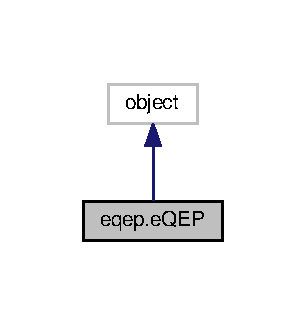
\includegraphics[width=147pt]{classeqep_1_1eQEP__inherit__graph}
\end{center}
\end{figure}


Collaboration diagram for eqep.\+e\+Q\+EP\+:
\nopagebreak
\begin{figure}[H]
\begin{center}
\leavevmode
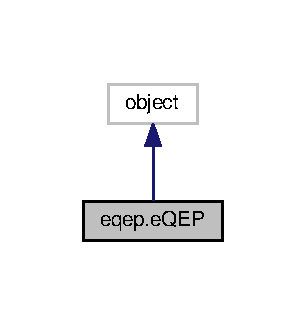
\includegraphics[width=147pt]{classeqep_1_1eQEP__coll__graph}
\end{center}
\end{figure}
\subsection*{Public Member Functions}
\begin{DoxyCompactItemize}
\item 
def \hyperlink{classeqep_1_1eQEP_ab214d60b7425c1d7803e3dff282b4255}{set\+\_\+mode} (self, mode)
\begin{DoxyCompactList}\small\item\em Set the mode of the \hyperlink{classeqep_1_1eQEP}{e\+Q\+EP} hardware. \end{DoxyCompactList}\item 
def \hyperlink{classeqep_1_1eQEP_a0b00fff3014216779db96333c76c41d9}{get\+\_\+mode} (self)
\begin{DoxyCompactList}\small\item\em Get the mode of the \hyperlink{classeqep_1_1eQEP}{e\+Q\+EP} hardware. \end{DoxyCompactList}\item 
def \hyperlink{classeqep_1_1eQEP_af025879aa5f70b38b8309de87c06df43}{set\+\_\+period} (self, period)
\begin{DoxyCompactList}\small\item\em Set the unit timer period of the \hyperlink{classeqep_1_1eQEP}{e\+Q\+EP} hardware. \end{DoxyCompactList}\item 
def \hyperlink{classeqep_1_1eQEP_a21826fd1f1b7524fe3883e25f619de1f}{get\+\_\+period} (self)
\begin{DoxyCompactList}\small\item\em Get the unit timer period of the \hyperlink{classeqep_1_1eQEP}{e\+Q\+EP} hardware. \end{DoxyCompactList}\item 
def \hyperlink{classeqep_1_1eQEP_a4cc40a4f3989be38ae46e427e09dfb04}{set\+\_\+position} (self, position)
\begin{DoxyCompactList}\small\item\em Set the current position of the encoder hardware. \end{DoxyCompactList}\item 
def \hyperlink{classeqep_1_1eQEP_aec4ddf0439a2df98e527b2963925d397}{get\+\_\+position} (self)
\begin{DoxyCompactList}\small\item\em Get the immediate position of the encoder hardware. \end{DoxyCompactList}\item 
def \hyperlink{classeqep_1_1eQEP_add267f1f55ca1e5fcef34b1a70db18a0}{poll\+\_\+position} (self)
\begin{DoxyCompactList}\small\item\em Poll the position, returns when new data is available. \end{DoxyCompactList}\item 
def \hyperlink{classeqep_1_1eQEP_a8110a8aae6998a20760af30020f894d2}{\+\_\+\+\_\+init\+\_\+\+\_\+} (self, path, mode)
\begin{DoxyCompactList}\small\item\em Constructor -\/ specify the path and the mode. \end{DoxyCompactList}\item 
def \hyperlink{classeqep_1_1eQEP_ac80fa9e08911c4260207aacc72541863}{\+\_\+\+\_\+del\+\_\+\+\_\+} (self)\hypertarget{classeqep_1_1eQEP_ac80fa9e08911c4260207aacc72541863}{}\label{classeqep_1_1eQEP_ac80fa9e08911c4260207aacc72541863}

\begin{DoxyCompactList}\small\item\em Deconstructor. \end{DoxyCompactList}\end{DoxyCompactItemize}
\subsection*{Public Attributes}
\begin{DoxyCompactItemize}
\item 
{\bfseries path}\hypertarget{classeqep_1_1eQEP_a1230ab18199a963f9d954777a2a336ca}{}\label{classeqep_1_1eQEP_a1230ab18199a963f9d954777a2a336ca}

\item 
{\bfseries fd}\hypertarget{classeqep_1_1eQEP_ac27da69238f8273eaf4e9883baec9aaa}{}\label{classeqep_1_1eQEP_ac27da69238f8273eaf4e9883baec9aaa}

\item 
{\bfseries poller}\hypertarget{classeqep_1_1eQEP_a3894927414d08b27680caa9580fd4776}{}\label{classeqep_1_1eQEP_a3894927414d08b27680caa9580fd4776}

\end{DoxyCompactItemize}
\subsection*{Static Public Attributes}
\begin{DoxyCompactItemize}
\item 
int {\bfseries M\+O\+D\+E\+\_\+\+A\+B\+S\+O\+L\+U\+TE} = 0\hypertarget{classeqep_1_1eQEP_adb87525577f901bdc4845d527dc87ed7}{}\label{classeqep_1_1eQEP_adb87525577f901bdc4845d527dc87ed7}

\item 
int {\bfseries M\+O\+D\+E\+\_\+\+R\+E\+L\+A\+T\+I\+VE} = 1\hypertarget{classeqep_1_1eQEP_a6e95fe57827b6139f29bfd352d6bdf08}{}\label{classeqep_1_1eQEP_a6e95fe57827b6139f29bfd352d6bdf08}

\end{DoxyCompactItemize}


\subsection{Detailed Description}
Classe permettant de gerer la position du moteur. 

\subsection{Constructor \& Destructor Documentation}
\index{eqep\+::e\+Q\+EP@{eqep\+::e\+Q\+EP}!\+\_\+\+\_\+init\+\_\+\+\_\+@{\+\_\+\+\_\+init\+\_\+\+\_\+}}
\index{\+\_\+\+\_\+init\+\_\+\+\_\+@{\+\_\+\+\_\+init\+\_\+\+\_\+}!eqep\+::e\+Q\+EP@{eqep\+::e\+Q\+EP}}
\subsubsection[{\texorpdfstring{\+\_\+\+\_\+init\+\_\+\+\_\+(self, path, mode)}{__init__(self, path, mode)}}]{\setlength{\rightskip}{0pt plus 5cm}def eqep.\+e\+Q\+E\+P.\+\_\+\+\_\+init\+\_\+\+\_\+ (
\begin{DoxyParamCaption}
\item[{}]{self, }
\item[{}]{path, }
\item[{}]{mode}
\end{DoxyParamCaption}
)}\hypertarget{classeqep_1_1eQEP_a8110a8aae6998a20760af30020f894d2}{}\label{classeqep_1_1eQEP_a8110a8aae6998a20760af30020f894d2}


Constructor -\/ specify the path and the mode. 


\begin{DoxyParams}{Parameters}
{\em path} & The path of the encoder \\
\hline
{\em mode} & The desired mode\+: 0 (M\+O\+D\+E\+\_\+\+A\+B\+S\+O\+L\+U\+TE), 1 (M\+O\+D\+E\+\_\+\+R\+E\+L\+A\+T\+I\+VE) \\
\hline
\end{DoxyParams}


\subsection{Member Function Documentation}
\index{eqep\+::e\+Q\+EP@{eqep\+::e\+Q\+EP}!get\+\_\+mode@{get\+\_\+mode}}
\index{get\+\_\+mode@{get\+\_\+mode}!eqep\+::e\+Q\+EP@{eqep\+::e\+Q\+EP}}
\subsubsection[{\texorpdfstring{get\+\_\+mode(self)}{get_mode(self)}}]{\setlength{\rightskip}{0pt plus 5cm}def eqep.\+e\+Q\+E\+P.\+get\+\_\+mode (
\begin{DoxyParamCaption}
\item[{}]{self}
\end{DoxyParamCaption}
)}\hypertarget{classeqep_1_1eQEP_a0b00fff3014216779db96333c76c41d9}{}\label{classeqep_1_1eQEP_a0b00fff3014216779db96333c76c41d9}


Get the mode of the \hyperlink{classeqep_1_1eQEP}{e\+Q\+EP} hardware. 

\begin{DoxyReturn}{Returns}
The mode of the e\+Qep hardware 
\end{DoxyReturn}
\index{eqep\+::e\+Q\+EP@{eqep\+::e\+Q\+EP}!get\+\_\+period@{get\+\_\+period}}
\index{get\+\_\+period@{get\+\_\+period}!eqep\+::e\+Q\+EP@{eqep\+::e\+Q\+EP}}
\subsubsection[{\texorpdfstring{get\+\_\+period(self)}{get_period(self)}}]{\setlength{\rightskip}{0pt plus 5cm}def eqep.\+e\+Q\+E\+P.\+get\+\_\+period (
\begin{DoxyParamCaption}
\item[{}]{self}
\end{DoxyParamCaption}
)}\hypertarget{classeqep_1_1eQEP_a21826fd1f1b7524fe3883e25f619de1f}{}\label{classeqep_1_1eQEP_a21826fd1f1b7524fe3883e25f619de1f}


Get the unit timer period of the \hyperlink{classeqep_1_1eQEP}{e\+Q\+EP} hardware. 

\begin{DoxyReturn}{Returns}
The period of the e\+Qep hardware 
\end{DoxyReturn}
\index{eqep\+::e\+Q\+EP@{eqep\+::e\+Q\+EP}!get\+\_\+position@{get\+\_\+position}}
\index{get\+\_\+position@{get\+\_\+position}!eqep\+::e\+Q\+EP@{eqep\+::e\+Q\+EP}}
\subsubsection[{\texorpdfstring{get\+\_\+position(self)}{get_position(self)}}]{\setlength{\rightskip}{0pt plus 5cm}def eqep.\+e\+Q\+E\+P.\+get\+\_\+position (
\begin{DoxyParamCaption}
\item[{}]{self}
\end{DoxyParamCaption}
)}\hypertarget{classeqep_1_1eQEP_aec4ddf0439a2df98e527b2963925d397}{}\label{classeqep_1_1eQEP_aec4ddf0439a2df98e527b2963925d397}


Get the immediate position of the encoder hardware. 

\begin{DoxyReturn}{Returns}
The immediate position of the encoder 
\end{DoxyReturn}
\index{eqep\+::e\+Q\+EP@{eqep\+::e\+Q\+EP}!poll\+\_\+position@{poll\+\_\+position}}
\index{poll\+\_\+position@{poll\+\_\+position}!eqep\+::e\+Q\+EP@{eqep\+::e\+Q\+EP}}
\subsubsection[{\texorpdfstring{poll\+\_\+position(self)}{poll_position(self)}}]{\setlength{\rightskip}{0pt plus 5cm}def eqep.\+e\+Q\+E\+P.\+poll\+\_\+position (
\begin{DoxyParamCaption}
\item[{}]{self}
\end{DoxyParamCaption}
)}\hypertarget{classeqep_1_1eQEP_add267f1f55ca1e5fcef34b1a70db18a0}{}\label{classeqep_1_1eQEP_add267f1f55ca1e5fcef34b1a70db18a0}


Poll the position, returns when new data is available. 

\begin{DoxyReturn}{Returns}
This position 
\end{DoxyReturn}
\index{eqep\+::e\+Q\+EP@{eqep\+::e\+Q\+EP}!set\+\_\+mode@{set\+\_\+mode}}
\index{set\+\_\+mode@{set\+\_\+mode}!eqep\+::e\+Q\+EP@{eqep\+::e\+Q\+EP}}
\subsubsection[{\texorpdfstring{set\+\_\+mode(self, mode)}{set_mode(self, mode)}}]{\setlength{\rightskip}{0pt plus 5cm}def eqep.\+e\+Q\+E\+P.\+set\+\_\+mode (
\begin{DoxyParamCaption}
\item[{}]{self, }
\item[{}]{mode}
\end{DoxyParamCaption}
)}\hypertarget{classeqep_1_1eQEP_ab214d60b7425c1d7803e3dff282b4255}{}\label{classeqep_1_1eQEP_ab214d60b7425c1d7803e3dff282b4255}


Set the mode of the \hyperlink{classeqep_1_1eQEP}{e\+Q\+EP} hardware. 


\begin{DoxyParams}{Parameters}
{\em mode} & The mode of the \hyperlink{classeqep_1_1eQEP}{e\+Q\+EP} hardware \\
\hline
\end{DoxyParams}
\index{eqep\+::e\+Q\+EP@{eqep\+::e\+Q\+EP}!set\+\_\+period@{set\+\_\+period}}
\index{set\+\_\+period@{set\+\_\+period}!eqep\+::e\+Q\+EP@{eqep\+::e\+Q\+EP}}
\subsubsection[{\texorpdfstring{set\+\_\+period(self, period)}{set_period(self, period)}}]{\setlength{\rightskip}{0pt plus 5cm}def eqep.\+e\+Q\+E\+P.\+set\+\_\+period (
\begin{DoxyParamCaption}
\item[{}]{self, }
\item[{}]{period}
\end{DoxyParamCaption}
)}\hypertarget{classeqep_1_1eQEP_af025879aa5f70b38b8309de87c06df43}{}\label{classeqep_1_1eQEP_af025879aa5f70b38b8309de87c06df43}


Set the unit timer period of the \hyperlink{classeqep_1_1eQEP}{e\+Q\+EP} hardware. 


\begin{DoxyParams}{Parameters}
{\em period} & The unit timer period of the \hyperlink{classeqep_1_1eQEP}{e\+Q\+EP} hardware \\
\hline
\end{DoxyParams}
\index{eqep\+::e\+Q\+EP@{eqep\+::e\+Q\+EP}!set\+\_\+position@{set\+\_\+position}}
\index{set\+\_\+position@{set\+\_\+position}!eqep\+::e\+Q\+EP@{eqep\+::e\+Q\+EP}}
\subsubsection[{\texorpdfstring{set\+\_\+position(self, position)}{set_position(self, position)}}]{\setlength{\rightskip}{0pt plus 5cm}def eqep.\+e\+Q\+E\+P.\+set\+\_\+position (
\begin{DoxyParamCaption}
\item[{}]{self, }
\item[{}]{position}
\end{DoxyParamCaption}
)}\hypertarget{classeqep_1_1eQEP_a4cc40a4f3989be38ae46e427e09dfb04}{}\label{classeqep_1_1eQEP_a4cc40a4f3989be38ae46e427e09dfb04}


Set the current position of the encoder hardware. 


\begin{DoxyParams}{Parameters}
{\em position} & The new position of the encoder hardware \\
\hline
\end{DoxyParams}


The documentation for this class was generated from the following file\+:\begin{DoxyCompactItemize}
\item 
eqep.\+py\end{DoxyCompactItemize}

\hypertarget{classpwm_1_1PWM}{}\section{pwm.\+P\+WM Class Reference}
\label{classpwm_1_1PWM}\index{pwm.\+P\+WM@{pwm.\+P\+WM}}


Classe permettant de gerer le module \hyperlink{classpwm_1_1PWM}{P\+WM}.  




Inheritance diagram for pwm.\+P\+WM\+:\nopagebreak
\begin{figure}[H]
\begin{center}
\leavevmode
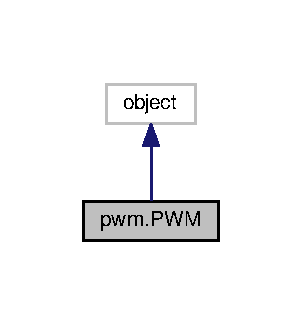
\includegraphics[width=145pt]{classpwm_1_1PWM__inherit__graph}
\end{center}
\end{figure}


Collaboration diagram for pwm.\+P\+WM\+:\nopagebreak
\begin{figure}[H]
\begin{center}
\leavevmode
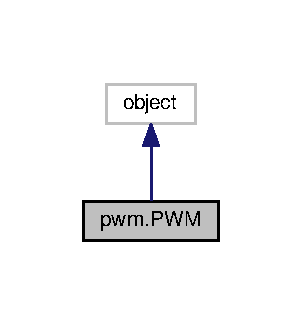
\includegraphics[width=145pt]{classpwm_1_1PWM__coll__graph}
\end{center}
\end{figure}
\subsection*{Public Member Functions}
\begin{DoxyCompactItemize}
\item 
def \hyperlink{classpwm_1_1PWM_aecbf9d1e49de6ac566cb2fc2166006b8}{set\+\_\+duty\+\_\+cycle} (self, pin\+P\+WM, duty\+\_\+cycle)
\begin{DoxyCompactList}\small\item\em Definit le duty\+\_\+cycle. \end{DoxyCompactList}\item 
def \hyperlink{classpwm_1_1PWM_ad9deb36402c7415728071e5cc9d00ef0}{set\+\_\+period} (self, pin\+P\+WM, period)
\begin{DoxyCompactList}\small\item\em Definit la periode du \hyperlink{classpwm_1_1PWM}{P\+WM}. \end{DoxyCompactList}\item 
def \hyperlink{classpwm_1_1PWM_aa911dffbe75afb2bbeca8f7cb4361e03}{\+\_\+\+\_\+init\+\_\+\+\_\+} (self)\hypertarget{classpwm_1_1PWM_aa911dffbe75afb2bbeca8f7cb4361e03}{}\label{classpwm_1_1PWM_aa911dffbe75afb2bbeca8f7cb4361e03}

\begin{DoxyCompactList}\small\item\em Constructor. \end{DoxyCompactList}\item 
def \hyperlink{classpwm_1_1PWM_a6e5d3baeb7ce9e250980638733bf62ef}{stop} (self, pin\+P\+WM)
\begin{DoxyCompactList}\small\item\em Envoie un duty\+\_\+cycle de 0. \end{DoxyCompactList}\end{DoxyCompactItemize}
\subsection*{Public Attributes}
\begin{DoxyCompactItemize}
\item 
{\bfseries period}\hypertarget{classpwm_1_1PWM_a97e8c6f96847cd6a4bf641b7da51dfe7}{}\label{classpwm_1_1PWM_a97e8c6f96847cd6a4bf641b7da51dfe7}

\item 
{\bfseries path}\hypertarget{classpwm_1_1PWM_a2caefbe7eb198384cf8538367e9f883f}{}\label{classpwm_1_1PWM_a2caefbe7eb198384cf8538367e9f883f}

\end{DoxyCompactItemize}


\subsection{Detailed Description}
Classe permettant de gerer le module \hyperlink{classpwm_1_1PWM}{P\+WM}. 

\subsection{Member Function Documentation}
\index{pwm\+::\+P\+WM@{pwm\+::\+P\+WM}!set\+\_\+duty\+\_\+cycle@{set\+\_\+duty\+\_\+cycle}}
\index{set\+\_\+duty\+\_\+cycle@{set\+\_\+duty\+\_\+cycle}!pwm\+::\+P\+WM@{pwm\+::\+P\+WM}}
\subsubsection[{\texorpdfstring{set\+\_\+duty\+\_\+cycle(self, pin\+P\+W\+M, duty\+\_\+cycle)}{set_duty_cycle(self, pinPWM, duty_cycle)}}]{\setlength{\rightskip}{0pt plus 5cm}def pwm.\+P\+W\+M.\+set\+\_\+duty\+\_\+cycle (
\begin{DoxyParamCaption}
\item[{}]{self, }
\item[{}]{pin\+P\+WM, }
\item[{}]{duty\+\_\+cycle}
\end{DoxyParamCaption}
)}\hypertarget{classpwm_1_1PWM_aecbf9d1e49de6ac566cb2fc2166006b8}{}\label{classpwm_1_1PWM_aecbf9d1e49de6ac566cb2fc2166006b8}


Definit le duty\+\_\+cycle. 


\begin{DoxyParams}{Parameters}
{\em pin\+P\+WM} & Le pin de \hyperlink{classpwm_1_1PWM}{P\+WM} \\
\hline
{\em duty\+\_\+cycle} & La valeur du duty\+\_\+cycle souhaite \\
\hline
\end{DoxyParams}
\index{pwm\+::\+P\+WM@{pwm\+::\+P\+WM}!set\+\_\+period@{set\+\_\+period}}
\index{set\+\_\+period@{set\+\_\+period}!pwm\+::\+P\+WM@{pwm\+::\+P\+WM}}
\subsubsection[{\texorpdfstring{set\+\_\+period(self, pin\+P\+W\+M, period)}{set_period(self, pinPWM, period)}}]{\setlength{\rightskip}{0pt plus 5cm}def pwm.\+P\+W\+M.\+set\+\_\+period (
\begin{DoxyParamCaption}
\item[{}]{self, }
\item[{}]{pin\+P\+WM, }
\item[{}]{period}
\end{DoxyParamCaption}
)}\hypertarget{classpwm_1_1PWM_ad9deb36402c7415728071e5cc9d00ef0}{}\label{classpwm_1_1PWM_ad9deb36402c7415728071e5cc9d00ef0}


Definit la periode du \hyperlink{classpwm_1_1PWM}{P\+WM}. 


\begin{DoxyParams}{Parameters}
{\em pin\+P\+WM} & Le pin de \hyperlink{classpwm_1_1PWM}{P\+WM} \\
\hline
{\em period} & La valeur de la periode souhaitee \\
\hline
\end{DoxyParams}
\index{pwm\+::\+P\+WM@{pwm\+::\+P\+WM}!stop@{stop}}
\index{stop@{stop}!pwm\+::\+P\+WM@{pwm\+::\+P\+WM}}
\subsubsection[{\texorpdfstring{stop(self, pin\+P\+W\+M)}{stop(self, pinPWM)}}]{\setlength{\rightskip}{0pt plus 5cm}def pwm.\+P\+W\+M.\+stop (
\begin{DoxyParamCaption}
\item[{}]{self, }
\item[{}]{pin\+P\+WM}
\end{DoxyParamCaption}
)}\hypertarget{classpwm_1_1PWM_a6e5d3baeb7ce9e250980638733bf62ef}{}\label{classpwm_1_1PWM_a6e5d3baeb7ce9e250980638733bf62ef}


Envoie un duty\+\_\+cycle de 0. 


\begin{DoxyParams}{Parameters}
{\em pin\+P\+WM} & Le pin de \hyperlink{classpwm_1_1PWM}{P\+WM} \\
\hline
\end{DoxyParams}


The documentation for this class was generated from the following file\+:\begin{DoxyCompactItemize}
\item 
pwm.\+py\end{DoxyCompactItemize}

\hypertarget{classwakanda_1_1Wakanda}{}\section{wakanda.\+Wakanda Class Reference}
\label{classwakanda_1_1Wakanda}\index{wakanda.\+Wakanda@{wakanda.\+Wakanda}}


Classe principale responsable du suivi de trajectoire.  




Inheritance diagram for wakanda.\+Wakanda\+:\nopagebreak
\begin{figure}[H]
\begin{center}
\leavevmode
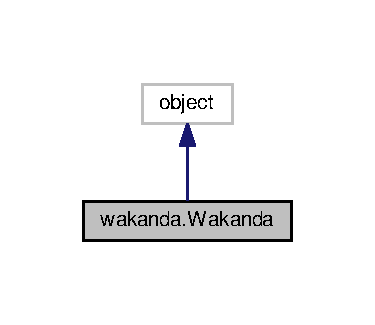
\includegraphics[width=180pt]{classwakanda_1_1Wakanda__inherit__graph}
\end{center}
\end{figure}


Collaboration diagram for wakanda.\+Wakanda\+:\nopagebreak
\begin{figure}[H]
\begin{center}
\leavevmode
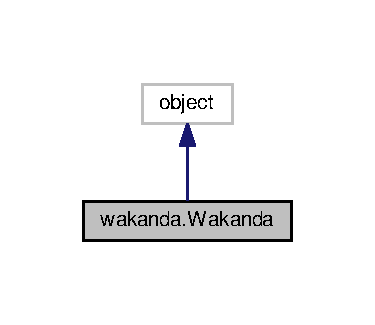
\includegraphics[width=180pt]{classwakanda_1_1Wakanda__coll__graph}
\end{center}
\end{figure}
\subsection*{Public Member Functions}
\begin{DoxyCompactItemize}
\item 
def \hyperlink{classwakanda_1_1Wakanda_a27ff7fb9ac3819931b93481588fb1e9f}{\+\_\+\+\_\+init\+\_\+\+\_\+} (self)\hypertarget{classwakanda_1_1Wakanda_a27ff7fb9ac3819931b93481588fb1e9f}{}\label{classwakanda_1_1Wakanda_a27ff7fb9ac3819931b93481588fb1e9f}

\begin{DoxyCompactList}\small\item\em Constructor. \end{DoxyCompactList}\item 
def \hyperlink{classwakanda_1_1Wakanda_a2240de179408dbc71c6892200cf5db1e}{modele\+Inverse} (self, x, y)
\begin{DoxyCompactList}\small\item\em Function computing the angular positions of the motors required to place the effector at (x,y) \end{DoxyCompactList}\item 
def \hyperlink{classwakanda_1_1Wakanda_a483ae1156569ce4c833611e5c688ed81}{is\+Reached} (self, error)
\begin{DoxyCompactList}\small\item\em Function verifying if the position targeted by the controller is reached with an given error. \end{DoxyCompactList}\end{DoxyCompactItemize}
\subsection*{Public Attributes}
\begin{DoxyCompactItemize}
\item 
{\bfseries controller}\hypertarget{classwakanda_1_1Wakanda_afa13c93d1acb04864ffb955670283f3f}{}\label{classwakanda_1_1Wakanda_afa13c93d1acb04864ffb955670283f3f}

\item 
{\bfseries og}\hypertarget{classwakanda_1_1Wakanda_aa8f99260cf4c31f0568aeabce94eb730}{}\label{classwakanda_1_1Wakanda_aa8f99260cf4c31f0568aeabce94eb730}

\item 
{\bfseries od}\hypertarget{classwakanda_1_1Wakanda_a0ffaac6b73ad8a383d669882bfaff80e}{}\label{classwakanda_1_1Wakanda_a0ffaac6b73ad8a383d669882bfaff80e}

\item 
{\bfseries l1}\hypertarget{classwakanda_1_1Wakanda_a0adce3e75ec43f53a88d3f8d52cc01e2}{}\label{classwakanda_1_1Wakanda_a0adce3e75ec43f53a88d3f8d52cc01e2}

\item 
{\bfseries l2}\hypertarget{classwakanda_1_1Wakanda_ac14b24f1212b25550698d56a861dc63a}{}\label{classwakanda_1_1Wakanda_ac14b24f1212b25550698d56a861dc63a}

\item 
{\bfseries positions}\hypertarget{classwakanda_1_1Wakanda_a968f66cd49217b9762b1eeaca9eeef74}{}\label{classwakanda_1_1Wakanda_a968f66cd49217b9762b1eeaca9eeef74}

\end{DoxyCompactItemize}


\subsection{Detailed Description}
Classe principale responsable du suivi de trajectoire. 


\begin{DoxyParams}{Parameters}
{\em period} & The unit timer period of the e\+Q\+EP hardware \\
\hline
\end{DoxyParams}


\subsection{Member Function Documentation}
\index{wakanda\+::\+Wakanda@{wakanda\+::\+Wakanda}!is\+Reached@{is\+Reached}}
\index{is\+Reached@{is\+Reached}!wakanda\+::\+Wakanda@{wakanda\+::\+Wakanda}}
\subsubsection[{\texorpdfstring{is\+Reached(self, error)}{isReached(self, error)}}]{\setlength{\rightskip}{0pt plus 5cm}def wakanda.\+Wakanda.\+is\+Reached (
\begin{DoxyParamCaption}
\item[{}]{self, }
\item[{}]{error}
\end{DoxyParamCaption}
)}\hypertarget{classwakanda_1_1Wakanda_a483ae1156569ce4c833611e5c688ed81}{}\label{classwakanda_1_1Wakanda_a483ae1156569ce4c833611e5c688ed81}


Function verifying if the position targeted by the controller is reached with an given error. 


\begin{DoxyParams}{Parameters}
{\em error} & Maximal value of the command to consider that the target for the controller is reached \\
\hline
\end{DoxyParams}
\begin{DoxyReturn}{Returns}
True if the position is reached, False otherwise 
\end{DoxyReturn}
\index{wakanda\+::\+Wakanda@{wakanda\+::\+Wakanda}!modele\+Inverse@{modele\+Inverse}}
\index{modele\+Inverse@{modele\+Inverse}!wakanda\+::\+Wakanda@{wakanda\+::\+Wakanda}}
\subsubsection[{\texorpdfstring{modele\+Inverse(self, x, y)}{modeleInverse(self, x, y)}}]{\setlength{\rightskip}{0pt plus 5cm}def wakanda.\+Wakanda.\+modele\+Inverse (
\begin{DoxyParamCaption}
\item[{}]{self, }
\item[{}]{x, }
\item[{}]{y}
\end{DoxyParamCaption}
)}\hypertarget{classwakanda_1_1Wakanda_a2240de179408dbc71c6892200cf5db1e}{}\label{classwakanda_1_1Wakanda_a2240de179408dbc71c6892200cf5db1e}


Function computing the angular positions of the motors required to place the effector at (x,y) 


\begin{DoxyParams}{Parameters}
{\em x,y} & Position of the effector \\
\hline
\end{DoxyParams}
\begin{DoxyReturn}{Returns}
An array containing the angles of the left and right motors. If the given position is unreachable, the function returns an empty array 
\end{DoxyReturn}


The documentation for this class was generated from the following file\+:\begin{DoxyCompactItemize}
\item 
wakanda.\+py\end{DoxyCompactItemize}

%--- End generated contents ---

% Index
\backmatter
\newpage
\phantomsection
\clearemptydoublepage
\addcontentsline{toc}{chapter}{Index}
\printindex

\end{document}
